%
%===============>>  ГРУППА 9-1 МОДУЛЬ 7  <<=============
%
\setmodule{7}

%BEGIN_FOLD % ====>>_____ Занятие 1 _____<<====
\begin{class}[number=1]
	\begin{definit}
		\textbf{Синусом} острого угла прямоугольного треугольника называется отношение противолежащего катета к гипотенузе.
	\end{definit}
	\begin{definit}
		\textbf{Косинусом} острого угла прямоугольного треугольника называется отношение прилежащего катета к гипотенузе.
	\end{definit}
	\begin{definit}
		\textbf{Тангенсом} острого угла прямоугольного треугольника называется отношение противолежащего катета к прилежащему катету.
	\end{definit}
	\begin{definit}
		\textbf{Основное тригонометрическое тождество:} \[\sin^2\alpha+\cos^2\alpha=1\]
	\end{definit}
	\begin{listofex}
		\item В треугольнике \( ABC \) угол \( C \) равен \( 90 \) градусов, \( AC=6 \), \( AB=20 \). Найдите \( \sin B \).
		\item  В треугольнике \( ABC \) угол \( C \) равен \( 90 \) градусов, \( BC=9 \), \( AB=20 \). Найдите \( \cos B \).
		\item В треугольнике \( ABC \) угол \( C \) равен \( 90 \) градусов, \( BC=9 \), \( AC=27 \). Найдите \( \tg B \).
		\item Найдите синус, косинус и тангенс углов \( A \) и \( B \) треугольника \( ABC \) с прямым углом \( C \), если:
		\begin{tasks}(2)
			\task \( BC=8 \), \( AB=17 \)
			\task \( BC=21 \), \( AC=20 \)
			\task \( BC=1 \), \( AC=2 \)
		\end{tasks}
		\item Найдите:
		\begin{tasks}(1)
			\task \( \sin\alpha \) и \( \tg\alpha \), если \( \cos\alpha=\dfrac{1}{2} \)
			\task \( \cos\alpha \) и \( \tg\alpha \), если \( \sin\alpha=\dfrac{\sqrt{3}}{2} \)
		\end{tasks}
		\item В треугольнике \( ABC \) угол \( C \) прямой, \( BC=8 \), \( \sin A=0,4 \). Найдите \( AB \).
		\item В треугольнике \( ABC \) угол \( C \) прямой, \( AC=15 \), \( \cos A=\dfrac{5}{7} \). Найдите \( AB \).
		\item В треугольнике \( ABC \) угол \( C \) равен \( 90\degree \), \( BC=12 \), \( \sin A=\dfrac{4}{11} \). Найдите \( AB \).
		\item Катеты прямоугольного треугольника равны \( \sqrt{15} \) и \( 1 \). Найдите синус наименьшего угла этого треугольника.
		\item Площадь прямоугольного треугольника равна \( 32\sqrt{3} \). Один из острых углов равен \( 30\degree \). Найдите длину гипотенузы.
		\item В треугольнике \( ABC \) угол \( C \) равен \( 90\degree \), \( AC=12 \), \( \tg A=\dfrac{2\sqrt{10}}{3} \).  Найдите \( AB \).
		\item В треугольнике \( ABC \) угол \( C \) равен \( 90\degree \), \( \sin A=\dfrac{4}{5} \), \( AC=9 \). Найдите \( AB \).
		\item Найдите синус меньшего острого угла между	диагональю прямоугольника и его стороной, если периметр прямоугольника равен \( 34 \) см, а одна из сторон --- \( 12 \) см. 
		\item Тангенс острого угла прямоугольного треугольника равен \( \dfrac{2}{5} \), а один из катетов на \( 6 \) см больше другого. Найдите площадь треугольника. 
		\item Основание равнобедренного треугольника равно \( 8 \) см, тангенс угла при основании равен \( 2 \). Найдите площадь треугольника. 
		\item Периметр равнобедренного треугольника равен \( 64 \) см, косинус угла при основании равен \( 0,6 \). Найдите площадь треугольника.
		\item Моторная лодка прошла \( 36 \) км по течению реки и вернулась обратно, потратив на весь путь \( 5 \) часов. Скорость течения реки равна \( 3 \) км/ч. Найдите скорость лодки в неподвижной воде.
		\item Баржа прошла по течению реки \( 48 \) км и, повернув обратно, прошла ещё \( 36 \) км, затратив на весь путь \( 6 \) часов. Найдите собственную скорость баржи, если скорость течения реки равна \( 5 \) км/ч.
		\item Теплоход проходит по течению реки до пункта назначения \( 280 \) км и после стоянки возвращается в пункт отправления. Найдите скорость теплохода в неподвижной воде, если скорость течения равна \( 4 \) км/ч, стоянка длится \( 15 \) часов, а в пункт отправления теплоход возвращается через \( 39 \) часов после отплытия из него.
	\end{listofex}
\end{class}
%END_FOLD

%BEGIN_FOLD % ====>>_____ Занятие 2 _____<<====
\begin{class}[number=2]
	\begin{listofex}
		\item В треугольнике \( ABC \) угол \( C \) равен \( 90\degree \), \( \sin A=\dfrac{4}{5} \), \( AC=9 \). Найдите \( AB \).
		\item Найдите синус меньшего острого угла между	диагональю прямоугольника и его стороной, если периметр прямоугольника равен \( 34 \) см, а одна из сторон --- \( 12 \) см. 
		\item Тангенс острого угла прямоугольного треугольника равен \( \dfrac{2}{5} \), а один из катетов на \( 6 \) см больше другого. Найдите площадь треугольника. 
		\item Основание равнобедренного треугольника равно \( 8 \) см, тангенс угла при основании равен \( 2 \). Найдите площадь треугольника. 
		\item Периметр равнобедренного треугольника равен \( 64 \) см, косинус угла при основании равен \( 0,6 \). Найдите площадь треугольника.
	\end{listofex}
		\begin{definit}
			\textbf{Теорема синусов}: Отношение длины стороны треугольника к синусу противолежащего угла равно двум радиусам описанной около треугольника окружности: \[\dfrac{a}{\sin\alpha}=\dfrac{b}{\sin\beta}=\dfrac{c}{\sin\gamma}=2R\]
		\end{definit}
		\begin{definit}
			\textbf{Теорема косинусов}: Квадрат любой стороны треугольника (\( a \)) равен сумме квадратов двух других сторон треугольника (\( b \) и \( c \)), минус удвоенное произведение этих сторон на косинус угла между ними: \[a^2=b^2+c^2-2bc\cos\alpha\]
		\end{definit}
	\begin{listofex}[resume]
		\item В треугольнике \( ABC \) известно, что \( AB=8 \), \( BC=10 \), \( AC=12 \). Найдите \( \cos\angle ABC \).
		\item Выяснить вид треугольника (остроугольный, прямоугольный, тупоугольный), если длины его сторон равны \( 23 \) см, \( 17 \) см, \( 19 \) см. 
		\item Стороны треугольника равны \( 8\sqrt{3} \) см, \( \sqrt{577} \) см и \( \sqrt{11} \) см. Найдите наибольший угол	этого треугольника. 
		\item Две стороны параллелограмма равны \( 4 \) см и \( 5 \) см, а одна из диагоналей --- \( 46 \)
		см. Найти вторую диагональ параллелограмма.
		\item В треугольнике \( ABC \) сторона \( AB \) равна \( 2\sqrt{3} \), угол \( C \) равен \( 120\degree \). Найдите радиус описанной около этого треугольника окружности.
		\item Сторона правильного треугольника равна \( \sqrt{3} \). Найдите радиус окружности, описанной около этого треугольника.
		\item Найдите хорду, на которую опирается угол \( 120\degree \), вписанный в окружность радиуса \( \sqrt{3} \).  
		\item Сторона \( AB \) треугольника \( ABC \) равна \( 1 \). Противолежащий ей угол \( C \) равен \( 120\degree \). Найдите радиус окружности, описанной около этого треугольника.
		\item Угол \( C \) треугольника \( ABC \), вписанного в окружность радиуса \( 3 \), равен \( 30\degree \). Найдите сторону \( AB \) этого треугольника.
		\item Одна сторона остроугольного треугольника равна радиусу описанной около него окружности. Найдите угол треугольника, противолежащий этой стороне. Ответ дайте в градусах.
		\item В треугольнике \( ABC \) угол \( B \) равен \( 72\degree \), угол \( C \) равен \( 63\degree \), \( BC=2\sqrt{2} \). Найдите радиус описанной около этого треугольника окружности.
		\item Моторная лодка прошла \( 36 \) км по течению реки и вернулась обратно, потратив на весь путь \( 5 \) часов. Скорость течения реки равна \( 3 \) км/ч. Найдите скорость лодки в неподвижной воде.
		\item Баржа прошла по течению реки \( 48 \) км и, повернув обратно, прошла ещё \( 36 \) км, затратив на весь путь \( 6 \) часов. Найдите собственную скорость баржи, если скорость течения реки равна \( 5 \) км/ч.
		\item Теплоход проходит по течению реки до пункта назначения \( 280 \) км и после стоянки возвращается в пункт отправления. Найдите скорость теплохода в неподвижной воде, если скорость течения равна \( 4 \) км/ч, стоянка длится \( 15 \) часов, а в пункт отправления теплоход возвращается через \( 39 \) часов после отплытия из него.
	\end{listofex}
\end{class}
%END_FOLD

%BEGIN_FOLD % ====>>_ Домашняя работа 1 _<<====
\begin{homework}[number=1]
	\begin{listofex}
		\item В треугольнике \( ABC \) угол \( C \) равен \( 90\degree \), \( AC=9 \), \( AB=25 \). Найдите \( \sin B \).
		\item В треугольнике \( ABC \) угол \( C \) равен \( 90\degree \), BC\( =4 \), \( AC=28 \). Найдите \( \tg B \).
		\item В треугольнике \( ABC \) угол \( C \) равен \( 90\degree \), \( \sin B=\dfrac{5}{17} \), \( AB=51 \). Найдите \( AC \).
		\item В треугольнике\( ABC \) угол \( C \) равен \( 90\degree \), \( \tg B=\dfrac{8}{5} \), \( BC=20 \). Найдите \( AC \).
		\item Синус острого угла \( A \) треугольника \( ABC \) равен \( \dfrac{2\sqrt{6}}{5} \). Найдите \( \cos A \).
		\item В равнобедренном треугольнике \( ABC \) \( AB=BC \). Угол \( B \) равен \( 120\degree \), а высота, опущенная на основание равна \( \dfrac{\sqrt{3}}{2} \). Найдите площадь треугольника.
		\item В треугольнике \( ABC \) известно, что \( AB=6 \), \( BC=7 \), \( AC=8 \). Найдите \( \cos\angle ABC \).
		\item В треугольнике \( ABC \) угол \( A \) равен \( 60\degree \), угол \( B \) равен \( 45\degree \), \( BC=5\sqrt{6} \). Найдите \( AC \).
		\item Сторона правильного треугольника равна \( 3 \). Найдите радиус окружности, описанной около этого треугольника.
	\end{listofex}
\end{homework}
%END_FOLD

%BEGIN_FOLD % ====>>_____ Занятие 3 _____<<====
\begin{class}[number=3]
	\begin{listofex}
		\item Найдите угол \( ABC \), изображенный на рисунке. Ответ дайте в градусах.
		\begin{center}
			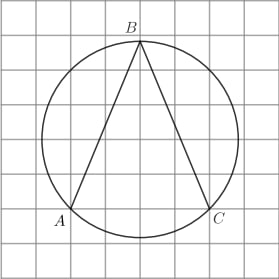
\includegraphics[align=t, width=0.3\linewidth]{\picpath/G92M7L2}
		\end{center}
		\item Найдите градусную меру дуги \( AC \) окружности, на которую опирается угол \( ABC \). Ответ
		дайте в градусах.
		\begin{center}
			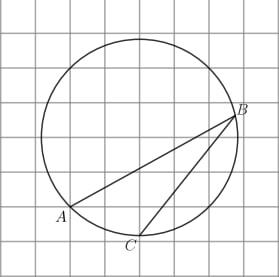
\includegraphics[align=t, width=0.3\linewidth]{\picpath/G92M7L2-2}
		\end{center}
		\item Найдите угол \( AOB \), изображенный на рисунке. Ответ дайте в градусах.
		\begin{center}
			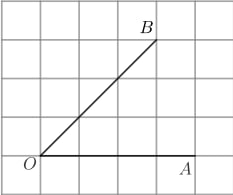
\includegraphics[align=t, width=0.3\linewidth]{\picpath/G92M7L2-3}
		\end{center}
		\item На клетчатой бумаге с размером клетки \( 1X1 \) изображён угол \( AOB \). Найдите его тангенс.
		\begin{center}
			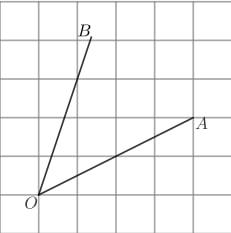
\includegraphics[align=t, width=0.3\linewidth]{\picpath/G92M7L2-4}
		\end{center}
		\item Моторная лодка прошла \( 36 \) км по течению реки и вернулась обратно, потратив на весь путь \( 5 \) часов. Скорость течения реки равна \( 3 \) км/ч. Найдите скорость лодки в неподвижной воде.
		\item Баржа прошла по течению реки \( 48 \) км и, повернув обратно, прошла ещё \( 36 \) км, затратив на весь путь \( 6 \) часов. Найдите собственную скорость баржи, если скорость течения реки равна \( 5 \) км/ч.
		\item Теплоход проходит по течению реки до пункта назначения \( 280 \) км и после стоянки возвращается в пункт отправления. Найдите скорость теплохода в неподвижной воде, если скорость течения равна \( 4 \) км/ч, стоянка длится \( 15 \) часов, а в пункт отправления теплоход возвращается через \( 39 \) часов после отплытия из него.
		\item Из пунктов \( A \) и \( B \), расстояние между которыми \( 19 \) км, вышли одновременно навстречу друг другу два пешехода и встретились в \( 9 \) км от \( A \). Найдите скорость пешехода, шедшего из \( A \), если известно, что он шёл со скоростью, на \( 1 \) км/ч большей, чем пешеход, шедший из \( B \), и сделал в пути получасовую остановку.
		\item Расстояние между городами \( A \) и \( B \) равно \( 750 \) км. Из города \( A \) в город \( B \) со скоростью \( 50 \) км/ч выехал первый автомобиль, а через три часа после этого навстречу ему из города \( B \) выехал со скоростью \( 70 \) км/ч второй автомобиль. На каком расстоянии от города \( A \) автомобили встретятся?
	\end{listofex}
\end{class}
%END_FOLD

%BEGIN_FOLD % ====>>_____ Занятие 4 _____<<====
\begin{class}[number=4]
	\begin{listofex}
		\item Упростите выражение:
			\[\dfrac{\sqrt{\sqrt{10}-2}\cdot\sqrt{\sqrt{10}+2}}{\sqrt{24}}\]
		\item Сократите дроби:
		\begin{tasks}(2)
			\task \( \dfrac{5^{n+1}-5^{n-1}}{2\cdot5^n} \)
			\task \( \dfrac{18^{n+3}}{3^{2n+5}\cdot2^{n-2}} \)
		\end{tasks}
		\item Катер прошёл от одной пристани до другой, расстояние между которыми по реке равно \( 48 \) км, сделал стоянку на \( 20 \) мин и вернулся обратно через \( \mfrac{5}{1}{3} \) ч после начала поездки. Найдите скорость течения реки, если известно, что скорость катера в стоячей воде равна \( 20 \) км/ч.
		\item Из пункта \( A \) в пункт \( B \), расположенный ниже по течению реки, отправился плот. Одновременно навстречу ему из пункта \( B \) вышел катер. Встретив плот, катер сразу повернул и поплыл назад. Какую часть пути от \( A \) до \( B \) пройдет плот к моменту возвращения катера в пункт \( B \), если скорость катера в стоячей воде вчетверо больше скорости течения реки?
		\item Расстояние между пристанями \( A \) и \( B \) равно \( 80 \) км. Из \( A \) в \( B \) по течению реки отправился плот, а через \( 2 \) часа вслед за ним отправилась яхта, которая, прибыв в пункт \( B \), тотчас повернула обратно и возвратилась в \( A \). К этому времени плот прошел \( 22 \) км. Найдите скорость яхты в неподвижной воде, если скорость течения реки равна \( 2 \) км/ч. Ответ дайте в км/ч.
		\item Расстояние между пристанями \( A \) и \( B \) равно \( 126 \) км. Из \( A \) в \( B \) по течению реки отправился плот, а через \( 1 \) час вслед за ним отправилась яхта, которая, прибыв в пункт \( B \), тотчас повернула обратно и возвратилась в \( A \). К этому времени плот прошел \( 34  \) км. Найдите скорость яхты в неподвижной воде, если скорость течения реки равна \( 2 \) км/ч. Ответ дайте в км/ч.
		\item Пристани \( A \) и \( B \) расположены на реке, скорость течения которой на этом участке равна \( 3 \) км/ч. Лодка проходит туда и обратно без остановок со средней скоростью \( 8 \) км/ч. Найдите собственную скорость лодки.
	\end{listofex}
\end{class}
%END_FOLD

%BEGIN_FOLD % ====>>_ Домашняя работа 2 _<<====
\begin{homework}[number=2]
	\begin{listofex}
		\item Сократите дробь: \[\dfrac{100^n}{5^{2n-1}\cdot4^{n-2}}\]
		\item Моторная лодка прошла против течения реки \( 132 \) км и вернулась в пункт отправления, затратив на обратный путь на \( 5 \) часов меньше, чем на путь против течения. Найдите скорость лодки в неподвижной воде, если скорость течения реки равна \( 5 \) км/ч.
		\item Расстояние между пристанями \( A \) и \( B \) равно \( 108 \) км. Из \( A \) в \( B \) по течению реки отправился плот, а через час вслед за ним отправилась моторная лодка, которая, прибыв в пункт \( B \), тотчас повернула обратно и возвратилась в \( A \). К этому времени плот прошёл \( 50 \) км. Найдите скорость лодки в неподвижной воде, если скорость течения реки равна \( 5 \) км/ч.
		\item Пристани \( A \) и \( B \) расположены на реке, скорость течения которой на этом участке равна \( 4 \) км/ч. Лодка проходит от \( A \) до \( B \) и обратно без остановок со средней скоростью \( 6 \) км/ч. Найдите собственную скорость лодки.
	\end{listofex}
\end{homework}
%END_FOLD

%BEGIN_FOLD % ====>>_____ Занятие 5 _____<<====
\begin{class}[number=5]
	\begin{listofex}
		\item Найдите значение выражения:
		\begin{tasks}(2)
			\task \( \dfrac{3^8\cdot3^5}{3^9} \)
			\task \( \dfrac{24^4}{3^2\cdot8^3} \)
			\task \( (3\sqrt{2})^2 \)
			\task \( 4^{-10}\cdot(4^3)^4 \)
			\task \( 3\cdot10^{-1}+1\cdot10^{-2}+5\cdot10^{-4} \)
			\task \( \dfrac{1}{4^{-10}}\cdot\dfrac{1}{4^{9}} \)
		\end{tasks}
		\item Из пунктов \( A \) и \( B \), расстояние между которыми \( 19 \) км, вышли одновременно навстречу друг другу два пешехода и встретились в \( 9 \) км от \( A \). Найдите скорость пешехода, шедшего из \( A \), если известно, что он шёл со скоростью, на \( 1 \) км/ч большей, чем пешеход, шедший из \( B \), и сделал в пути получасовую остановку.
		\item Расстояние между городами \( A \) и \( B \) равно \( 750 \) км. Из города \( A \) в город \( B \) со скоростью \( 50 \) км/ч выехал первый автомобиль, а через три часа после этого навстречу ему из города \( B \) выехал со скоростью \( 70 \) км/ч второй автомобиль. На каком расстоянии от города \( A \) автомобили встретятся?
		\item Из пункта \( A \) в пункт \( B \), расстояние между которыми \( 13 \) км, вышел пешеход. Одновременно с ним из \( B \) в \( A \) выехал велосипедист. Велосипедист ехал со скоростью, на \( 11 \) км/ч большей скорости пешехода, и сделал в пути получасовую остановку. Найдите скорость пешехода, если известно, что они встретились в \( 8 \) км от пункта \( B \).
		\item Два велосипедиста одновременно отправляются в \( 60 \)-километровый пробег. Первый едет со скоростью на \( 10 \) км/ч большей, чем второй, и прибывает к финишу на \( 3 \) часа раньше второго. Найдите скорость велосипедиста, пришедшего к финишу вторым.
		\item Велосипедист выехал с постоянной скоростью из города \( A \) в город \( B \), расстояние между которыми равно \( 60 \) км. Отдохнув, он отправился обратно в \( A \), увеличив скорость на \( 10 \) км/ч. По пути он сделал остановку на \( 3 \) часа, в результате чего затратил на обратный путь столько же времени, сколько на путь из \( A \) в \( B \). Найдите скорость велосипедиста на пути из \( A \) в \( B \).
	\end{listofex}
\end{class}
%END_FOLD

%BEGIN_FOLD % ====>>_____ Занятие 6 _____<<====
\begin{class}[number=6]
	\begin{listofex}
		\item Сократите дроби:
		\begin{tasks}(2)
			\task \( \dfrac{(2a^2)^3\cdot(3b)^2}{(6a^3b)^2} \)
			\task \( \dfrac{(3x)^3\cdot x^{-9}}{x^{-10}\cdot2x^4} \)
		\end{tasks}
		\item Первые \( 5 \) часов автомобиль ехал со скоростью \( 60 \) км/ч, следующие \( 3 \) часа --- со скоростью \( 100 \) км/ч, а последние \( 4 \) часа --- со скоростью \( 75 \) км/ч. Найдите среднюю скорость автомобиля на протяжении всего пути.
		\item Первые \( 300 \) км автомобиль ехал со скоростью \( 60 \) км/ч, следующие \( 300 \) км --- со скоростью \( 100 \) км/ч, а последние \( 300 \) км --- со скоростью \( 75 \) км/ч. Найдите среднюю скорость автомобиля на протяжении всего пути.
		\item Из \( A \) в \( B \) одновременно выехали два автомобилиста. Первый проехал с постоянной скоростью весь путь. Второй проехал первую половину пути со скоростью \( 30 \) км/ч, а вторую половину пути проехал со скоростью, большей скорости первого на \( 9 \) км/ч, в результате чего прибыл в \( В \) одновременно с первым автомобилистом. Найдите скорость первого автомобилиста.
		\item Первый велосипедист выехал из посёлка по шоссе со скоростью \( 21 \) км/ч. Через час после него со скоростью \( 15 \) км/ч из того же посёлка в том же направлении выехал второй велосипедист, а ещё через час --- третий. Найдите скорость третьего велосипедиста, если сначала он догнал второго, а через \( 9 \) часов после этого догнал первого.
		\item Два бегуна одновременно стартовали в одном направлении из одного и того же места круговой трассы в беге на несколько кругов. Спустя один час, когда одному из них оставалось \( 1 \) км до окончания первого круга, ему сообщили, что второй бегун прошёл первый круг \( 15 \) минут назад. Найдите скорость первого бегуна, если известно, что она на \( 6 \) км/ч меньше скорости второго.
		\item Два автомобиля одновременно отправляются в \( 420 \)-километровый пробег. Первый едет со скоростью, на \( 24 \) км/ч большей, чем второй, и прибывает к финишу на \( 2 \) ч раньше второго. Найдите скорость первого автомобиля.
	\end{listofex}
\end{class}
%END_FOLD

%BEGIN_FOLD % ====>>_ Домашняя работа 3 _<<====
\begin{homework}[number=3]
	\begin{listofex}
		\item Упростите выражение:
		\[\dfrac{18^n}{3^{2n-1}\cdot2^{n-2}}\]
		\item Из пункта \( A \) в пункт \( B \), расстояние между которыми \( 27 \) км, вышел турист. Через полчаса навстречу ему из пункта \( B \) вышел пешеход и встретил туриста в \( 12 \) км от \( A \). Найдите скорость туриста, если известно, что она была на \( 2 \) км/ч меньше скорости пешехода.
		\item Рыболов в \( 5 \) часов утра на моторной лодке отправился от пристани против течения реки, через некоторое время бросил якорь, \( 2 \) часа ловил рыбу и вернулся обратно в \( 10 \) часов утра того же дня. На какое расстояние от пристани он отдалился, если скорость реки равна \( 2 \) км/ч, а собственная скорость лодки \( 6 \) км/ч?
		\item Первые \( 2 \) часа автомобиль ехал со скоростью \( 70 \) км/ч, следующие \( 3 \) часа --- со скоростью \( 65 \) км/ч, а последние \( 3 \) часа --- со скоростью \( 75 \) км/ч. Найдите среднюю скорость автомобиля на протяжении всего пути.
	\end{listofex}
\end{homework}
%END_FOLD

%BEGIN_FOLD % ====>>_____ Занятие 7 _____<<====
\begin{class}[number=7]
	\begin{listofex}
		\item Решите неравенства:
		\begin{tasks}(2)
			\task \( \dfrac{x^2}{3}<\dfrac{3x+3}{4} \)
			\task \( \dfrac{11x-4}{5}\ge\dfrac{x^2}{2} \)
		\end{tasks}
		\item Упростите выражение:
		\[\dfrac{6}{a-1}-\dfrac{10}{(a-1)^2}:\dfrac{10}{a^2-1}-\dfrac{2a+2}{a-1}\]
		\item При смешивании первого раствора кислоты, концентрация которого \( 30\% \), и второго раствора этой же кислоты, концентрация которого \( 50\% \), получили раствор, содержащий \( 45\% \) кислоты. В каком отношении были взяты первый и второй растворы?
		\item Имеется два сплава с разным содержанием меди: в первом содержится \( 60\% \), а во втором --- \( 45\% \) меди. В каком отношении надо взять первый и второй сплавы, чтобы получить из них новый сплав, содержащий \( 55\% \) меди?
		\item Смешали некоторое количество \( 19 \)-процентного раствора некоторого вещества с таким же количеством \( 23 \)-процентного раствора этого же вещества. Сколько процентов составляет концентрация получившегося раствора?
		\item Туристы проплыли на лодке от лагеря некоторое расстояние вверх по течению реки, затем причалили к берегу и, погуляв \( 3 \) часа, вернулись обратно через \( 5 \) часов от начала путешествия. На какое расстояние от лагеря они отплыли, если скорость течения реки равна \( 3 \) км/ч, а собственная скорость лодки \( 9 \) км/ч?
	\end{listofex}
\end{class}
%END_FOLD

=%BEGIN_FOLD % ====>>_ Проверочная работа _<<====
\begin{exam}
	\begin{listofex}
		\item Проверочная
	\end{listofex}
\end{exam}
%END_FOLD

%BEGIN_FOLD % ====>>_ Консультация _<<====
\begin{consultation}
	\begin{listofex}
		\item Решите уравнение:
		\[(2x-2)^2(x-2)=(2x-2)(x-2)^2\]
		\item Решите неравенства:
		\begin{tasks}(2)
			\task \( \dfrac{-14}{x^2+2x-15}\le0 \)
			\task \( \dfrac{-10}{(x-3)^2}\ge0 \)
			\task \( (x-7)^2<\sqrt{11}(x-7) \)
			\task \( (\sqrt{3}-1,5)(3-2x)>0 \)
		\end{tasks}
		\item При смешивании первого раствора кислоты, концентрация которого \( 20\% \), и второго раствора этой же кислоты, концентрация которого \( 50\% \), получили раствор, содержащий \( 30\% \) кислоты. В каком отношении были взяты первый и второй растворы?
		\item Имеется два сплава с разным содержанием меди: в первом содержится \( 60\% \), а во втором -- \( 45\% \) меди. В каком отношении надо взять первый и второй сплавы, чтобы получить из них новый сплав, содержащий \( 55\% \) меди?
		\item Смешали некоторое количество \( 21 \)-процентного раствора некоторого вещества с таким же количеством \( 95 \)-процентного раствора этого же вещества. Сколько процентов составляет концентрация получившегося раствора?
		\item Первый сплав содержит \( 5\% \) меди, второй --- \( 13\% \) меди. Масса второго сплава больше массы первого на \( 4 \) кг. Из этих двух сплавов получили третий сплав, содержащий \( 10\% \) меди. Найдите массу третьего сплава.
		\item Два оператора, работая вместе, могут набрать текст газеты объявлений за \( 8 \) ч. Если первый оператор будет работать \( 3 \) ч, а второй \( 12 \) ч, то они выполнят только \( 75\% \) всей работы. За какое время может набрать весь текст каждый оператор, работая отдельно?
		\item Дима и Саша выполняют одинаковый тест. Дима отвечает за час на \( 12 \) вопросов теста, а Саша --- на \( 22 \). Они одновременно начали отвечать на вопросы теста, и Дима закончил свой тест позже Саши на \( 75 \) минут. Сколько вопросов содержит тест?
		\item Две трубы наполняют бассейн за \( 6 \) часов \( 18 \) минут, а одна первая труба наполняет бассейн за \( 9 \) часов. За сколько часов наполняет бассейн одна вторая труба?
		\item Постройте график функции
		\[y=	 \left\{
		\begin{array}{l}
			2x-2, \quad x<3\\
			-3x+13 \quad 3\leq x\leq4\\
			1,5x-7, \quad x>4.
		\end{array}
		\right. \]
		Определите, при каких значениях \( m \) прямая \( y=m \) имеет с графиком ровно две общие точки.
		\item Постройте график функции
		\[y=	 \left\{
		\begin{array}{l}
			x^2+2x+3, \quad x\leq-3,\\
			x+9, \quad x>-3
		\end{array}
		\right. \]
		и определите, при каких значениях \( m \) прямая \( y=m \) имеет с графиком ровно две общие точки.
	\end{listofex}
\end{consultation}
%END_FOLD